\setcounter{framenumber}{224}
\begin{frame}
  \LectureNo{8}
  \maketitle
\end{frame}

\begin{frame}{Overview}
\tableofcontents
\end{frame}

\section{Rehash}
\begin{frame}{Rehash}
	
\begin{itemize}

	\item Now we move to first-order logic.
	
	\item Propositional logic deals with inferences involving the sentential connectives ``not,'' ``and,'' ``or,'' \dots; \alert{first-order logic also allows for the quantifiers ``for all'' and ``there exists.''}

	\item We start with syntax:
	
		\begin{itemize}
		
			\item \alert{We model ordinary language by means of formal languages, artificial languages whose grammar is given by precise mathematical rules.}

		
		\end{itemize}
	
\end{itemize}

\end{frame}
		

\section{8. Syntax of First-Order Logic}
\subsection{8.1 First-Order Languages}

\begin{frame}{8.1 First-Order Languages}

	\begin{itemize}
		
		\item (8.1.1) Remember that in first-order (f.o.) logic we deal with the quantifiers ``for all'' and ``there is'':
		
		\begin{enumerate}[(1)]
		\setcounter{enumii}{2}
	
		\item This ball is scarlet and everything that's scarlet is red. So, this ball is red.
		
		\item The letter is in the left drawer. So there is something in the left drawer.
	
	\end{enumerate}
	
	\item In propositional logic, we can't accurately handle these inferences:
	\[p,q\nvDash r\]
	\[p\nvDash q\]
		
	\item (8.1.2) We need to take into account the \emph{internal grammatical structure} of sentences:
		\[\underbrace{\text{The ball}}_{\text{Term}}~\underbrace{\text{is scarlet}}_{\text{Predicate}}\]
		
	\end{itemize}

\end{frame}

\begin{frame}{Abstraction}

	\begin{itemize}
	
		\item The concrete terms and predicates don't matter:
				\begin{enumerate}[(1')]
		\setcounter{enumii}{2}
	
		\item This train is slow and everything that's slow is yellow. So, this train is yellow.
		
		\item The dog is in the car. So there is something in the car.
	
	\end{enumerate}

	\item So, we can abstract away from them:
		
			\begin{itemize}
			
				\item Terms: $t,u,v,\mathellipsis$
				
				\item Predicates: $P,R,Q,\mathellipsis$
			
			\end{itemize}
			
	\item We get:
	
		\begin{itemize}
		
			\item The ball is red $\leadsto$ $P(t)$
			
			\item The letter is in the left drawer $\leadsto$ $R(t,u)$
		
		\end{itemize}

	
	\end{itemize}

\end{frame}

\begin{frame}{Kinds of Terms}

	\begin{itemize}
	
		\item (8.1.3) In classical f.o. logic, we distinguish \emph{three} kinds of terms:
		
		\begin{itemize}
		
			\item \emph{proper names}, like ``Johannes'' or ``Angela'' (constants)
			
			\item \emph{pronouns}, like ``he,'' ``she,'' and ``it'' (variables)
			
			\item \emph{functional terms}, like ``the birthplace of Ada Lovelace'' or ``the LCA of Ada Lovelace and Alan Turing'' (\dots functions)
		
		\end{itemize}
		
		\item We use:
		
			\begin{itemize}
			
				\item $a,b,c,\mathellipsis$ as constants
				
				\item $x,y,z,\mathellipsis$ as variables
				
				\item $f,g,h,\mathellipsis$ as function symbols
			
			\end{itemize}
			
		\item (8.1.4) Note that functions can be \emph{nested}:
		
			\begin{itemize}
			
				\item[] The LCA of Ada Lovelace and the LCA of Alan Turing and Angela Merkel
				
				\item[$\leadsto$]  $f(a,f(b,c))$ 
			
			\end{itemize}
	
	\end{itemize}

\end{frame}

\begin{frame}{Quantifiers}

	\begin{itemize}
	
		\item (8.1.6) Enter the \emph{quantifiers} ``for all'' and ``there is'' (+ \dots):
		
		\begin{itemize}
		\item[] Everything that's scarlet is red.
		\item[$\leadsto$] Every $\underbrace{\text{object}}_{\text{indefinite}}$ is such that if $\underbrace{\text{it}}_{\text{pronoun}}$ is scarlet, then $\underbrace{\text{it}}_{\text{pronoun}}$ is red.
		\item[$\leadsto$] Every $x$ is such that if $x$ is scarlet, then $x$ is red.
		\end{itemize}
		
		\item We use the \emph{universal quantifier} $\forall$ for ``every'': 
	
		\begin{itemize}
		\item[$\leadsto$] $\forall x(S(x)\to R(x))$
		\end{itemize}
	
		\item (8.1.7) Similarly, we use the universal quantifier $\exists$ for ``there is'':
		
		\begin{itemize}
		
			\item[] There is something in the left drawer
			\item[$\leadsto$] There is some $\underbrace{\text{object}}_{\text{indefinite}}$ such that $\underbrace{\text{it}}_{\text{pronoun}}$ is in the left drawer
			\item[$\leadsto$] There is some $x$ such that $x$ is in the left drawer
			
			\item[$\leadsto$] $\exists xR(x,b)$
			
		\end{itemize}
	
	\end{itemize}

\end{frame}

\begin{frame}{Summary}

\begin{tabular}{c | l | l}
	Symbol & Name & Reading\\\hline
	$a,b,c,\mathellipsis$ & Constants & Proper names\\
	$x,y,z,\mathellipsis$ & Variables & Pronouns\\
	$f,g,h, \mathellipsis$ & Function symbols & Functional expressions\\
	$P,Q,R,\mathellipsis$ & Predicate symbols & Properties, relations\\
	$\forall $ & Universal quantifier & every, for all, each, \dots\\
	$\exists$ & Existential quantifier & there exists, for some, \dots
	\end{tabular}


\end{frame}

\subsection{8.2 Terms and Formulas}
\begin{frame}{8.2 Terms and Formulas}

	\begin{itemize}
	
		\item (8.2.1) A \emph{signature} is a structure $\mathcal{S}=(\mathcal{C}, \mathcal{F}, \mathcal{R}, ar)$ such that:
		\begin{enumerate}[(i)]
		
			\item $\mathcal{C}$ is a set of \emph{constant symbols}
			
			\item $\mathcal{F}$ is a set of \emph{function symbols}
			
			\item $\mathcal{R}$ is a set of \emph{predicate symbols}
			
			\item $ar:\mathcal{F}\cup\mathcal{R}\to\mathbb{N}$ is a function that assigns to each function and predicate symbol a fixed natural number, it's \emph{arity}
		\end{enumerate}

	\item (8.2.2) Notation:
	
		\begin{itemize}
		
			\item $R^n\in\mathcal{R}$ means $R\in\mathcal{R}$ with $ar(R)=n$
			\item $f^n\in\mathcal{F}$ means $f\in\mathcal{F}$ with $ar(f)=n$
		
		\end{itemize}
	
	\end{itemize}

\end{frame}

\begin{frame}{(8.2.3) Examples}

	\begin{enumerate}[(i)]
			
				\item $\mathcal{S}_{PA}=(\{0\}, \{S^1, +^2, \cdot^2\}, \alert{\emptyset})$ 
				
				\item $\mathcal{S}_\emptyset=(\alert{\emptyset},\alert{\emptyset},\alert{\emptyset})$
				
				\item $\mathcal{S}_\in=(\{\emptyset\}, \emptyset, \{\in^2\})$
			
			
				\item$\mathcal{S}=(\{a,b,c\}, \{f^1, g^2\}, \{P^1, R^2\})$			
			\end{enumerate}	

\end{frame}

\begin{frame}{Logical Vocabulary}

	\begin{itemize}
	
		\item (8.2.4) The \emph{logical} vocabulary of every f.o. language is the same:
		\begin{enumerate}[(i)]
		
			\item the set of \emph{variables}: $\mathcal{V}=\{x,y,z,\mathellipsis\}$
			
			\item the \emph{sentential operators}: $\neg,\land,\lor,\to,\leftrightarrow$
			
			\item the \emph{identity predicate}: \alert{$=^2$}
			
			\item the \emph{quantifiers}: $\forall,\exists$
			
			\item the \emph{parentheses}: $(,)$.
		
		\end{enumerate}

		\item Note the distinguished, binary \emph{identity predicate} $=$.
		
		\item We don't abstract away from identity:
		
			\begin{itemize}
			
				\item[] The birthplace of Ada Lovelace and Alan Turing is the same.
				
				\item[$\leadsto$] $f(a)=f(b)$
				
				\item[\alert{Not}] $R(f(a),f(b))$
			
			\end{itemize}
	
	\end{itemize}

\end{frame}

\begin{frame}{The Recursive Definition of Terms}

	\begin{itemize}
	
		\item Because of function nesting, we need to define terms recursively
	
		\item (8.2.5). The set $\mathcal{T}$ of \emph{terms} is recursively defined as the smallest set $X$ such that:
		\begin{enumerate}[(i)]
		
			\item \begin{enumerate}[(a)]
			\item $\mathcal{V}\subseteq X$
			\item $\mathcal{C}\subseteq X$
			\end{enumerate}
			\item If $t_1, \mathellipsis, t_n\in X$ and $f\in\mathcal{F}$ with $ar(f)=n$, then $f(t_1, \mathellipsis, t_n)\in X$
	
	\end{enumerate}
	
		\item So, the terms are all the variables and constants plus the functional combinations of those.
		
	\end{itemize}

\end{frame}

\begin{frame}{(8.2.6) Examples}

	\begin{enumerate}[(i)]
			
				\item In $\mathcal{S}_{PA}$: \[S(0),S(S(0)),\mathellipsis\in\mathcal{T}\]\[S(x), S(y), +(0,0), \cdot(0,0), \cdot (Sx, +(0,0)),\mathellipsis\in\mathcal{T}\]	
				
				\item[] Notational conventions in $\mathcal{S}_{PA}$: 
				\begin{enumerate}[(a)]
					
					\item ${n}$ means $\underbrace{S(\mathellipsis S(0)\mathellipsis)}_{n\text{ times}}$: $1=S(0),2=S(S(0)),\mathellipsis$
					
					\item We use ``infix notation:''  $(2\cdot 4)={\cdot}(2,4), (2+ 4)={+}(2,4),$ etc.
					
					\item[] 
					
					\item[] But watch out for parentheses: $((2\cdot 4)+1)\neq (2\cdot (4+1))$
				\end{enumerate}
			
				\item In $\mathcal{S}_\emptyset$: only $x,y,z,\mathellipsis.$
				
				\item In $\mathcal{S}_\in$: only $\emptyset$ and $x,y,z,\mathellipsis.$				
				\item Assuming that $f^2\in\mathcal{F}$, we have \[f(x,x), f(x,y), f(y,x), f(y,y), f(f(x,y), f(y,x)),\mathellipsis\in\mathcal{T}\]
			\end{enumerate}


\end{frame}

\begin{frame}{The Recursive Definition of Formulas}

	\begin{itemize}
	
		\item (8.2.8) The set $\mathcal{L}$ of \emph{formulas} is recursively defined as the smallest set $X$ such that:
		\begin{enumerate}[(i)]
		
			\item \begin{enumerate}[(a)]
			
				\item If $R^n\in\mathcal{P}$ and $t_1, \mathellipsis, t_n\in \mathcal{T},$ then $R(t_1, \mathellipsis, t_n)\in X$.
				
				\item If $t_1,t_2\in \mathcal{T}$, then $t_1=t_2\in X$
				
				\end{enumerate}
			
			\item \begin{enumerate}[(a)]
			
				\item if $\phi\in X$, then $\neg \phi\in X$
				
				\item if $\phi,\psi\in X$, then $(\phi\circ\psi)\in X$ for $\circ=\land,\lor,\to,\leftrightarrow$
				
				\item if $\phi\in X$ and $x\in \mathcal{V}$, then $Qx\phi\in X$ for $Q=\exists,\forall$
			
			\end{enumerate}
							
		\end{enumerate}
		
		\item $R(t_1, \mathellipsis, t_n)$ and $t_1=t_2$ are called \emph{atomic formulas}.
		
		\item $t_1\neq t_2$ means $\neg{t_1=t_2}$

	
	\end{itemize}

\end{frame}

\begin{frame}{(8.2.10.i) Examples}

Formulas in $\mathcal{L}_{PA}$:
					\[x=10\]
					\[S(x)=44\]
					\[2+2=4\]
					\[1\cdot1=0\]
					\[\forall x S(x)\neq 0\]
					\[((2\cdot 2)=5\land S(44)=7)\]
					\[\forall x\forall y(x\neq y\to S(x)\neq S(y))\]
					\[\forall x\forall y(S(x)=y+1\to S(x)=S(y))\]
					\[\forall x\exists yS(x)=y\]


\end{frame}

\begin{frame}{(8.2.10.ii) Examples}

Formulas in $\mathcal{L}_\emptyset$:
				
				\[x=y\]
				\[(x=y\land y\neq z)\]
				\[\forall x\exists y(x=y\land \forall z y\neq z)\]
				\[\forall x\exists y x\neq y\]
				\[\exists x\exists y(x\neq y\land \forall z(z=x\lor z=y))\]

\end{frame}

\begin{frame}{(8.2.10.iii) Examples}

Formulas in $\mathcal{L}_\in$:
				\[{\in}(x,x)\]
				\[\forall x{\in}(\emptyset,x)\]
				\[\neg\exists x{\in}(x,\emptyset)\]
				\[\forall x({\in}(x,y)\to {\in}(x,z))\]
				\[\forall x\forall(x=y\leftrightarrow\forall z({\in}(z,x)\leftrightarrow {\in}(z,y))) \]			
				
Convention: $t\in u$ means ${\in}(t,u)$
\[x\in x\]
				\[\forall x~\emptyset\in x\]
				\[\neg\exists x~x\in \emptyset\]
				\[\forall x(x\in y\to x\in z)\]
				\[\forall x\forall y(x=y\leftrightarrow \forall z(z\in x\leftrightarrow z\in y))\]

\end{frame}

\begin{frame}{(8.2.10.iv) Examples}

Formulas in $\mathcal{L}$ over $\mathcal{S}=(\{a,b,c\}, \{f^1, g^2\}, \{P^1, R^2\})$:
				
				\[R(f(g(a,b)),g(f(a),f(b)))\]
				\[\forall x P(f(a))\]
				\[\forall x(P(a)\to \exists yR(x,y))\]
				\[(\forall xP(x)\land \forall xQ(x))\]
				\[\forall x(P(x)\lor \forall xQ(x))\]
				\[(P(x)\leftrightarrow \forall y\forall xR(x,y))\]

\end{frame}

\begin{frame}{Induction on $\mathcal{L}$}

	\begin{itemize}
	
		\item \textbf{Theorem}. Let $\Phi$ be a condition on formulas. If we can show:
		\begin{enumerate}[(i)]
		
			\item  \begin{enumerate}[(a)]
			
				\item $\Phi(R(t_1,\mathellipsis, t_n))$ for all $R^n\in \mathcal{R}$ and $t_1,\mathellipsis, t_n\in\mathcal{T}$
				
				\item $\Phi(t_1=t_2)$ for $t_1,t_2\in \mathcal{T}$
			
			\end{enumerate}
			
			\item \begin{enumerate}[(a)]
			
			\item For all $\phi\in\mathcal{L}$, if $\Phi(\phi)$, then $\Phi(\neg\phi)$.

			\item For all $\phi,\psi\in\mathcal{L}$, if $\Phi(\phi)$ and $\Phi(\psi)$, then $\Phi((\phi\circ\psi))$, for $\circ=\land,\lor,\to,\leftrightarrow$.
			
			\item For all $\phi\in\mathcal{L}$, if $\Phi(\phi)$, then $\Phi(Qx\phi)$ for $Q=\forall,\exists$.

		
		\end{enumerate}
		\end{enumerate}
		Then we can conclude that for all $\phi\in\mathcal{L}$, $\Phi(\phi)$. 

	\item \textbf{Theorem}.  Let $\Phi$ be a condition on terms. If we can show:
		\begin{enumerate}[(i)]
		
			\item  \begin{enumerate}[(a)]
			
				\item $\Phi(a)$ for all $a\in\mathcal{C}$
				
				\item $\Phi(x)$ for all $x\in\mathcal{V}$
			
			\end{enumerate}
			
			\item If $\Phi(t_1), \mathellipsis,\Phi(t_n),$ then $\Phi(f(t_1,\mathellipsis,t_n))$.
		\end{enumerate}
		Then we can conclude that for all $t\in\mathcal{T}$, $\Phi(t)$.
	
	\end{itemize}


\end{frame}

\begin{frame}{(8.2.15) Recursion on $\mathcal{L}$}

We define $c:\mathcal{T}\to\mathbb{N}$ by:

	\begin{enumerate}[(i)]
	
		\item \begin{enumerate}[(a)]

			\item $c(a)=0$ for all $a\in\mathcal{C}$
			
			\item $c(x)=0$ for all $x\in \mathcal{V}$
	
			\end{enumerate}
			
		\item $c(f(t_1, \mathellipsis, t_n))=max(c(t_1), \mathellipsis, c(t_n))+1$
	
	\end{enumerate}

We define $c:\mathcal{L}\to\mathbb{N}$ by:
		\begin{enumerate}[(i)]
		
			\item  \begin{enumerate}[(a)]
			
				\item $c(R(t_1,\mathellipsis, t_n))=max(c(t_1), \mathellipsis, c(t_n))$
				
				\item $c(t_1=t_2)=max(c(t_1), c(t_2))$ 			
			\end{enumerate}
			
			\item \begin{enumerate}[(a)]
			
			\item $c(\neg\phi)=c(\phi)+1$
			\item $c(\phi\circ\psi)=max(c(\phi),c(\psi))+1$, for $\circ=\land,\lor,\to,\leftrightarrow$.
			
			\item $c(Qx\phi)=c(\phi)+1$ for $Q=\forall,\exists$.

		
		\end{enumerate}
		\end{enumerate}

\end{frame}

\subsection{8.3 Parsing Trees and Occurrences}
\begin{frame}{8.3 Parsing Trees and Occurrences}

	\begin{itemize}
	
		\item (8.3.2) We recursively define $T$, which assigns to $t\in\mathcal{T}$ its parsing tree:
		
\begin{center}
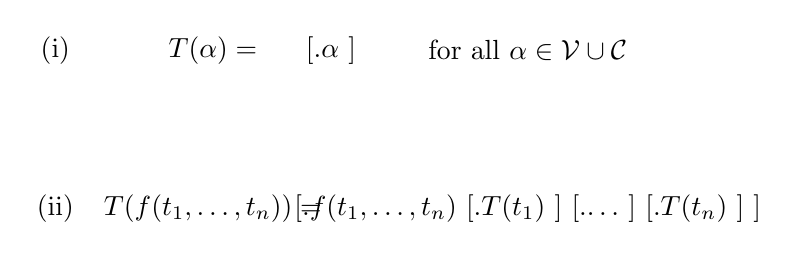
\begin{tikzpicture}
\node at (-2,1) {(i)};

\node at (0,1) {$T(\alpha)=$};
\node at (1.5,1) {\Tree [.$\alpha$ ]};
\node at (4,1) {for all $\alpha\in\mathcal{V}\cup\mathcal{C}$};

\node at (-2,-1) {(ii)};
\node at (0,-1) {$T(f(t_1, \mathellipsis,t_n))=$};
\node at (4,-1) {\Tree [.{$f(t_1, \mathellipsis,t_n)$} [.{$T(t_1)$} ] [.$\mathellipsis$ ] [.{$T(t_n)$} ] ]};

\end{tikzpicture}
\end{center}

	
	\end{itemize}

\end{frame}

\begin{frame}{(8.3.3) Examples}

	\begin{center}
			\begin{tabular}{c c}
			$4$ & $(2\cdot (2+1))$\\[2ex]
			\Tree [.$S(S(S(S(0))))$ [.$S(S(S(0)))$ [.$S(S(0))$ [.$S(0)$ [.$0$ ] ] ] ] ]
				
				&
				
					\Tree [.$(S(S(0))\cdot (S(S(0))+S(0)))$ [.$S(S(0))$ [.$S(0)$ [.$0$ ] ] ] [.$(S(S(0))+S(0))$ [.$S(S(0))$ [.$S(0)$ [.$0$ ] ]  ] [.$S(0)$ [.$0$ ] ] ] ]
			\end{tabular}
		\end{center}
				
	

\end{frame}

\begin{frame}{(8.3.4) Parsing Trees for Formulas}

{\small
\begin{center}
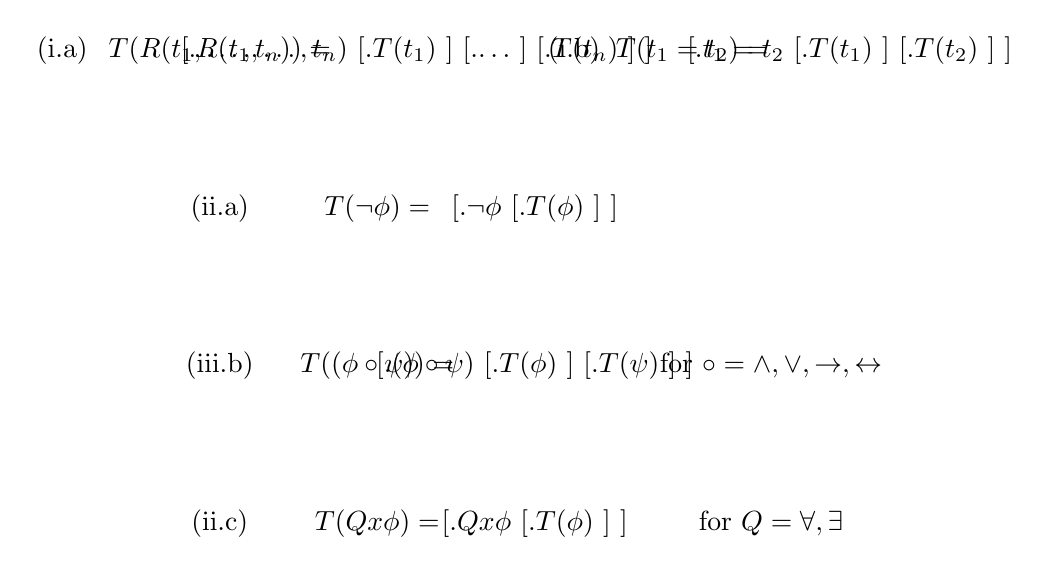
\begin{tikzpicture}
\node at (-4,1) {(i.a)};

\node at (-2,1) {$T(R(t_1, \mathellipsis, t_n))=$};
\node at (0.5,1) {\Tree [.{$R(t_1, \mathellipsis,t_n)$} [.{$T(t_1)$} ] [.$\mathellipsis$ ] [.{$T(t_n)$} ] ]};

\node at (2.5,1) {(i.b)};
\node at (4,1) {$T(t_1=t_2)=$};
\node at (6,1) {\Tree [.$t_1=t_2$ [.$T(t_1)$ ] [.$T(t_2)$ ] ]};

\node at (-2,-1) {(ii.a)};
\node at (0,-1) {$T(\neg \phi)=$};
\node at (2,-1) {\Tree [.$\neg \phi$ [.$T(\phi)$ ] ]};

\node at (-2,-3) {(iii.b)};
\node at (0,-3) {$T((\phi\circ\psi))=$};
\node at (2,-3) {\Tree [.$(\phi\circ\psi)$ [.$T(\phi)$ ] [.$T(\psi)$ ] ]};
\node at (5,-3) {for $\circ=\land,\lor,\to,\leftrightarrow$};


\node at (-2,-5) {(ii.c)};
\node at (0,-5) {$T(Qx \phi)=$};
\node at (2,-5) {\Tree [.$Qx\phi$ [.$T(\phi)$ ] ]};
\node at (5,-5) {for $Q=\forall,\exists$};


\end{tikzpicture}
\end{center}}

\end{frame}

\begin{frame}{(8.3.5) Example}

\begin{center}
	
	\Tree [.{$\forall x(R(x,g(f(a),f(b)))\to \exists yR(y,y))$} [.{$R(x,g(f(a),f(b)))\to \exists yR(y,y)$} [.{$R(x,g(f(a),f(b)))$} [.$x$ ] [.{$g(f(a),f(b))$} [.$f(a)$ [.$a$ ]  ] [.$f(b)$ [.$a$ ]  ] ] ] [.$\exists yR(y,y)$ [.$R(y,y)$ [.$y$ ]  [.$y$ ] ] ] ] ]
	
	\end{center}

\end{frame}

\begin{frame}{(8.3.7)  Stripped Parsing Trees via Example (8.3.8)}

\begin{center}
	
	\begin{tabular}{c c c}
	
	\Tree [.{$\forall x(R(x,g(f(a),f(b)))\to \exists yR(y,y))$} [.{$R(x,g(f(a),f(b)))\to \exists yR(y,y)$} [.{$R(x,g(f(a),f(b)))$} [.$x$ ] [.{$g(f(a),f(b))$} [.$f(a)$ [.$a$ ]  ] [.$f(b)$ [.$a$ ]  ] ] ] [.$\exists yR(y,y)$ [.$R(y,y)$ [.$y$ ]  [.$y$ ] ] ] ] ]
	
	&
	
	\Tree [.{$\forall x$} [.{$\to$} [.{$R$} [.$x$ ] [.{$g$} [.$f$ [.$a$ ]  ] [.$f$ [.$a$ ]  ] ] ] [.$\exists y$ [.$R$ [.$y$ ]  [.$y$ ] ] ] ] ]
	
	\end{tabular}
	
	\end{center}

\end{frame}

\begin{frame}{(8.3.9) Naming Nodes}

Take the tree:
		
			\begin{center}
				\Tree [.$\bullet$ [.$\bullet$  [.$\bullet$ [.$\bullet$ ] ] [.$\bullet$ [.$\bullet$ ] [.$\bullet$ ] ] ] ]
			\end{center}

	\begin{itemize}
		
		\item The root is always called $r$.
		
		\item The first child of the root is called $( r, 1)$.
		
		\item The first child of $( r, 1)$ is called $( r, 1, 1)$.
		
		\item The \emph{second} child of $( r, 1)$ is called $( r, 1, 2)$.
		
		\item The node $( r, 1, 1, 2)$ doesn't exist in our tree.
		
		\item Nodes: {\small$\{r, ( r,1), ( r,1,1), ( r,1,2),( r,1,1, 1), ( r,1,2,1), ( r,1,2,2)\}.$}
	
		\item We name a node by giving the ``directions'' for someone traveling along the edges through the nodes.	
	\end{itemize}

\end{frame}

\begin{frame}{Occurrences}

{\small
\begin{itemize}
	
		\item (8.3.10) An expression $\sigma$ \emph{occurs} in a term or formula $\tau$ iff $\sigma$ is the label of some node in the (ordinary or stripped) parsing tree of $\tau$.
	
	\item (8.3.11.iii) \emph{Example}. $R(x,y)$ occurs at $(r,1,2)$ and at $(r,1,2,1,1,2,1)$ in: 
\begin{center}{\tiny
\begin{tabular}{c}
\begin{tikzpicture}[level distance = 3em]
{\Tree [.$\forall x(R(x,y)\to \exists x\forall y(R(y,x)\land \neg R(x,y)))$
		[.$R(x,y)\to \exists x\forall y(R(y,x)\land \neg R(x,y))$ 
			[.\alert{$R(x,y)$} [.$x$ ] [.$y$ ] ]
			[.$\exists x\forall y(R(y,x)\land \neg R(x,y))$ 
				[.$\forall y(R(y,x)\land \neg R(x,y))$ 
					[.$R(y,x)\land \neg R(x,y)$ 
						[.$R(y,x)$
							[.$y$ ]
							[.$x$ ]
						]	
						[.$\neg R(x,y)$ 
							[.\alert{$R(x,y)$}
								[.$x$ ]
								[.$y$ ]
							]
						]
					]
				]
			]
		]
	]
}
\end{tikzpicture}
\end{tabular}}
\end{center}

	\item We define an \emph{occurrence} of $\sigma$ in $\phi$ as a pair $(n,\sigma)$ where $n$ is a node in the parsing tree labelled with $\sigma$.
	
	\end{itemize}
}

\end{frame}

\subsection{8.4 Free and Bound Variables}
\begin{frame}{8.4 Free and Bound Variables}

	\begin{itemize}
	
		\item (8.4.1) We want to understand the quantificational structure of formulas.
		
		\item (8.4.2) The quantifier $\forall x$ at $r$ in $\forall x(P(a)\land \neg R(x,a))$ captures $x$ at $(r,1,2,1,1)$.
		
		\item (8.4.4) In $\forall x({N}(x)\to {\exists x}R(x,x))$, $\forall x$ at $r$ binds $x$ at $(r,1,1,1)$, but \emph{not} at $(r,1,2,1,1)$ and  $(r,1,2,1,2)$.
		
		\begin{center}
		\Tree [.\alert{$\forall x$} [.$\to$ [.${N}$ [.\alert{$x$} ] ] [.${\color{green}\exists x}$ [.$R$ [.{\color{green}$x$} ] [.{\color{green}$x$} ] ] ] ] ]
		\end{center}
	
	\end{itemize}

\end{frame}

\begin{frame}{Variable Binding}

\begin{itemize}


	\item (8.4.5) Let $( n, x)$ be an occurrence of a variable $x$ in a formula $\phi$ and $( m, Qy)$ an occurrence of a quantifier $Q=\forall,\exists$ in $\phi$. Then, $( n, x)$ is {\it bound} by  $( m, Qy)$ iff
\begin{enumerate}[(i)]
\item $x=y,$
\item there is an downwards path from $m$ to $n,$
\item this path from $m$ to $n$ does not go through a node $k$ such that $( k, Q'x)$ is an occurrence of a quantifier $Q'=\forall,\exists$ in $\phi$.

\end{enumerate}
A variable occurrence that is not bound by any quantifier occurrence is \emph{free}.

\item \emph{Example}: $\forall x(\exists y \neg R(x,y)\lor (P(x)\to R(c,y)))$
	
	\begin{center}{\small
	\begin{tikzpicture}[level distance = 2em]
	 \Tree [.\alert{$\forall x$} [.$\lor$ [.{\color{green}$\exists y$} [.$\neg$ [.$R$ [.$\alert{x}$ ] [.{\color{green} $y$} ] ] ] ] [.$\to$ [.$P$ [.$\alert{x}$ ] ] [.$R$ [.$c$ ] [.{\color{blue}$y$} ] ] ] ] ]
	 \end{tikzpicture}}
	 \end{center}

\end{itemize}

\end{frame}

\begin{frame}{Example (8.4.6.iii)}


\begin{center}{\small
$\forall x(R(x,y)\to \exists x\forall y(R(y,x)\land \neg R(x,y)))$

\vspace{2ex}

\begin{tabular}{c}
\begin{tikzpicture}[level distance = 2em]
{\Tree [.{\color{red}$\forall x$}
		[.$\to$ 
			[.{$R$} [.{\color{red}$x$} ] [.{\color{purple}$y$} ] ]
			[.{\color{green}$\exists x$ }
				[.{\color{blue}$\forall y$} 
					[.$\land$ 
						[.$R$
							[.{\color{blue}$y$} ]
							[.{\color{green}$x$} ]
						]	
						[.$\neg$ 
							[.{$R$}
								[.{\color{green}$x$} ]
								[.{\color{blue}$y$} ]
							]
						]
					]
				]
			]
		]
	]
}
\end{tikzpicture}
\end{tabular}}
\end{center}

\end{frame}

\begin{frame}{Open and Closed Formulas}

	\begin{itemize}
	
		\item (8.4.7) A formula $\phi$ is open iff there is a free variable occurrence in it; otherwise $\phi$ is closed. Closed formulas are called \emph{sentences}.
		
		\item (8.4.8) \emph{Examples}:
		
		\begin{itemize}
			
				\item $\forall x(R(x,y)\to \exists x\forall y(R(y,x)\land \neg R(x,y)))$ is open, since $((r,1,1,2),y)$ is free.

			
				\item $\forall x(\exists y \neg R(x,y)\lor (P(x)\to R(c,y)))$ is open since $( ( r,1,2,2,2), y)$ is free
				
				\item $\forall x({N}(x)\to {\exists x}R(x,x))$ is closed.
			
			\end{itemize}
			
		
		\item (8.4.9) Open formulas don't have a definite truth-value, only sentcenes do.
		
		
	\end{itemize}

\end{frame}
\subsection{8.5 Substitution}
\begin{frame}{8.5 Substitution}

	\begin{itemize}
	
	
		\item (8.5.1) \emph{Substitution in Terms}. We define $(s)[x:=t]$ recursively by:
		
		\begin{enumerate}[(i)]
			
				\item $(s)[x:=t]=\begin{cases} s & \text{if } s\neq x\\ t & \text{ if }s=x\end{cases}$ for $s\in \mathcal{C}\cup\mathcal{V}$
				
				\item $(f(t_1,\mathellipsis, t_n))[x:=t]=f((t_1)[x:=t], \mathellipsis, (t_n)[x:=t])$
			
			\end{enumerate} 
			
			
		\item (8.5.2)  \emph{Substitution in Forulas}. We define $(\phi)[x:=t]$ (the result of substituting $t$ for all \emph{free} occurrences of $x$ in $\phi$) recursively as follows:
	
	
		\begin{enumerate}[(i)]
	
			\item \begin{enumerate}[(a)] 
			
				\item $(R(t_1, \mathellipsis, t_n))[x:=t]=R((t_1)[x:=t], \mathellipsis, (t_n)[x:=t])$
				
				\item $(t_1=t_2)[x:=t]=t_1[x:=t]=t_2[x:=t]$
				
			\end{enumerate}
			
			\item \begin{enumerate}[(a)] 

			\item $(\neg\phi)[x:=t]=\neg(\phi[x:=t])$

			
			\item $((\phi\circ\psi))[x:=t]=((\phi)[x:=t]\circ(\psi)[x:=t])$ for $\circ=\land,\lor,\to,\leftrightarrow$
			
			\item $(Qy\phi)[x:=t]=\begin{cases} Qy(\phi)[x:=t] & \text{if } y\neq x\\ Qy\phi & \text{if }y=x\end{cases}$ for $Q=\forall,\exists$

			\end{enumerate}
	

			\end{enumerate}
	
	\end{itemize}

\end{frame}

\begin{frame}{Example (8.5.4)}

$(\forall x(\exists y \neg R(x,y)\lor (P(x)\to R(c,y))))[y:=c]$
	\begin{align*}
	&=\forall x((\exists y \neg R(x,y)\lor (P(x)\to R(c,y))))[y:=c]\\
	&=\forall x(((\exists y \neg R(x,y)))[y:=c]\lor (((P(x)\to R(c,y))))[y:=c])\\
	&=\forall x((\exists y \neg R(x,y))\lor ((P(x))[y:=c]\to (R(c,y))[y:=c]))\\
	&=\forall x((\exists y \neg R(x,y))\lor (P((x)[y:=c])\to (R((c)[y:=c]), (y)[y:=c])))\\
	&=\forall x(\exists y \neg R(x,y)\lor (P(x)\to R(c,c)))
	\end{align*}

\end{frame}

\subsection{8.6 Formalization}
\begin{frame}{8.6 Formalization}

\begin{itemize}

	\item (8.6.1) The \emph{translation key} interprets the signature:
	
	\begin{enumerate}[(i)]
		
			\item A so-called \emph{domain of discourse}, $D$, which is the set of things we're talking about.
			
			\item For each constant in the signature, a natural language term it formalizes.
			
			\item For each predicate in the signature, a natural language predicate it formalizes.
			
			\item For each function symbol in the language, a natural language expression it formalizes.
			
		\end{enumerate}


\end{itemize}

\end{frame}

\begin{frame}{(8.6.3) Formalization Guidelines $\exists$}

\begin{tabular}{p{6.5cm} c l}
		
		Somebody who's smart exists & $\leadsto$ & $\exists x S(x)$\\

		
		There's somebody who's not smart & $\leadsto$ & $\exists x\neg S(x)$\\

Somebody's smart and somebody's handsome & $\leadsto$ & $\exists xS(x)\land \exists xH(x)$\\

Somebody's smart and handsome & $\leadsto$ & $\exists x(S(x)\land H(x))$\\
 Nobody's both smart and handsome & $\leadsto$ &$\neg\exists x(S(x)\land H(x))$\\
 
 Somebody, who's smart, is handsome & $\leadsto$ & $\exists x(S(x)\land H(x))$
		
		\end{tabular}
		
		\vspace{4ex}
		
		 \[\alert{\exists x(S(x)\to H(x))}\]

\end{frame}

\begin{frame}{(8.6.4) Formalization Guidelines $\forall$}

\begin{tabular}{p{6cm} c l}
		
		Not everybody handsome is smart & $\leadsto$ & $\neg\forall x(H(x)\to S(x))$\\
Everybody who's smart is handsome & $\leadsto$ &$\forall x(S(x)\to H(x))$\\
A person who's smart is handsome & $\leadsto$ &$\forall x(S(x)\to H(x))$\\
Someone who's smart is handsome & $\leadsto$ &$\forall x(S(x)\to H(x))$\\
Everybody's smart and handsome & $\leadsto$ &$\forall x(S(x)\land H(x))$
		\end{tabular}
		
		\vspace{4ex}
		
		\[\alert{\forall x(P(x)\to S(c))\neq \forall xP(x)\to S(c)}\]
		
		\[\alert{\forall x(P(x)\land S(x))\neq \forall x(P(x)\to S(x))}\]

\end{frame}

\begin{frame}{(8.6.5) Formalization Guidelines $x,y,z,\mathellipsis$}

Variables ``are'' pronouns:

\vspace{4ex}

\begin{tabular}{p{6cm} c l}
		He's handsome & $\leadsto$ & $H(x)$\\
		She's handsome and smart & $\leadsto$ & $H(x)\land S(x)$\\
		He's handsome and \emph{he}'s smart & $\leadsto$ & $H(x)\land S(y)$\\
		He's handsome and she's smart & $\leadsto$ & $H(x)\land S(y)$\\
		That's a smart and handsome gal & $\leadsto$ & $H(x)\land S(x)$\\
		
		
		\end{tabular}

\end{frame}

\begin{frame}{(8.6.7) Numerical Quantifiers}

\[\exists xP(x)\tag{Exists$_1$}\]
\[\forall x\forall y(P(x)\land P(y)\to x=y)\tag{At Most$_1$}\]
\[\exists x(P(x)\land \forall y(P(y)\to x=y))\tag{Exactly$_1$}\]

\[\exists x\exists y(P(x)\land P(y)\land x\neq y)\tag{Exists$_2$}\]
\[\forall x\forall y\forall z(P(x)\land P(y)\land P(z)\to x=y\lor x=z\lor y=z)\tag{At Most$_2$}\]
\[\exists x\exists y(P(x)\land P(y)\land \forall z(P(z)\to x=z\lor y=z))\tag{Exactly$_2$}\]
\end{frame}

\begin{frame}{Core Ideas (Lecture Version)}

	\begin{itemize}
	
		\item In f.o. logic, we take the grammatical structure of simple sentences into account.
		
		\item  Singular terms stand for objects, predicates for properties/relations.
		
		\item Quantifiers allow us talk about things in generality.
		
		\item The signature consists of a set of constants, of function symbols, and of predicate symbols each.
		
		\item Both terms and formulas are defined inductively in f.o.r logic.
		
		\item We have induction for formulas and terms and function recursion.
		
		\item Parsing trees are defined for terms and functions.
		
		\item Nodes in trees have a canonical way of being named: by the directions for how to find them starting at the root. 
		
		\item Variables are bound by quantifiers.
		
		\item A formula without free variables is closed, a sentence.
		
		\item Just like in propositional logic, there are guidelines for formalization.
					
	\end{itemize}

\end{frame}


\begin{frame}

	\begin{center}
	{\huge\bf Thanks!}
	\end{center}

\end{frame}

